\chapter{基于信息熵的数据定价研究}

\section{研究动机}
近些年来,数据量的巨幅增长,尤其是从2005年到2010年,全球产生的数据量增长了10倍(从130艾字节增长到了1227艾字节),目前仍在继续增长\cite{gantz2012digital,villars2011big}。数据交易的市场也以惊人的速度发展着,预计从目前到2020年,大数据和其商业分析的市场规模会从1301亿美元增长到2030亿美元\cite{idc}。如今,高质量和可信赖的数据商品及其相关的分析业务有着巨量的市场需求\cite{gantz2012digital,maitland2002european,turner2014digital,villars2011big}。

现在,数据商品和相关分析业务主要是由在线数据市场提供的。这些市场从数据发布者和全球网络收集数据,并对其进行清洗、挖掘和整理,然后出售给不同的消费者。具体来说,数据消费者主要由开发者和中小企业主构成。这些数据消费者需要在线数据市场提供的数据和相关分析业务来帮助他们做商业决策。至于在线数据市场,他们在整理过的、有价值的数据的基础上,提供分析、商业应用和算法等服务给消费者。现在,国外主要有三家数据交易平台,分别是Microsoft Windows Azure Data Marketplace\cite{MicrosoftAzure}, Inforchimps\cite{infochimps}以及Factual\cite{factual}。而国内也主要有三家平台,分别是贵阳大数据交易所\cite{gbdex},武汉长江大数据交易中心和武汉东湖大数据交易中心\cite{chinadatatrading}。然而,在这些国内外数据交易平台,并没有一个统一的定价机制来指导整个市场。因此,当前数据产品的定价处于一个比较混乱的阶段。不同的数据交易平台采用的是不同的定价机制,而其中最普遍采用的有四种种机制:基于订阅的定价机制、基于查询的定价机制,捆绑销售定价机制以及私下协商定价机制。选择什么样的定价机制具体取决于消费者使用模式以及数据提供商之间的竞争差异。但是,需要指出的是,目前没有任何一种定价机制将数据本身所含有的信息量考虑为定价因素。从消费者角度考虑,目前很多数据消费者通常只对市场上数据集的某些子集感兴趣,他们并不需要购买完整的数据集,而交易平台往往给出的是完整数据集的价格。当消费者购买这些子集时,他们需要知道这些子集所含信息占完整数据集的比例从而评估交易平台给出的子集定价是否合理。从数据交易平台的角度看,如果他们能给出更多的子集数据价格以及它们之间的信息量关系的话,就能给消费者提供一个更加透明的定价关系,从而吸引更多的消费者进行消费。另一方面,目前已有的定价机制并不能产生最大交易剩余,这样会降低买卖双方的交易信心,从而使原本能发生的交易而没有发生,这将会对数据及其相关交易带来极大的经济损失。因此,我们进行了基于信息熵的数据交易的研究课题,期望以数据产品本身的信息量作为定价指标来更好地指导数据交易。

\section{定价策略与模型}

在本小节中,我们首先会给出基于信息熵数据定价的问题定义。然后针对这一问题,提出了基于信息熵数据定价的通用模型,并讨论了相关的性质和应用范围。

\subsection{问题定义}

如今,大部分工业界收集到的数据都是非结构化的。即使这些非结构化的数据能用矩阵形式表示,但是人们还是很难从这些数据结构中认识到结构化的信息和信息分布。因此,我们很难真正认识到手中数据所蕴含的价值,所以也很难为其定一个合理的价格。这里,我们给出一个的士司机行驶数据集的例子来说明这一问题。

\begin{figure}[h]
  \centering
    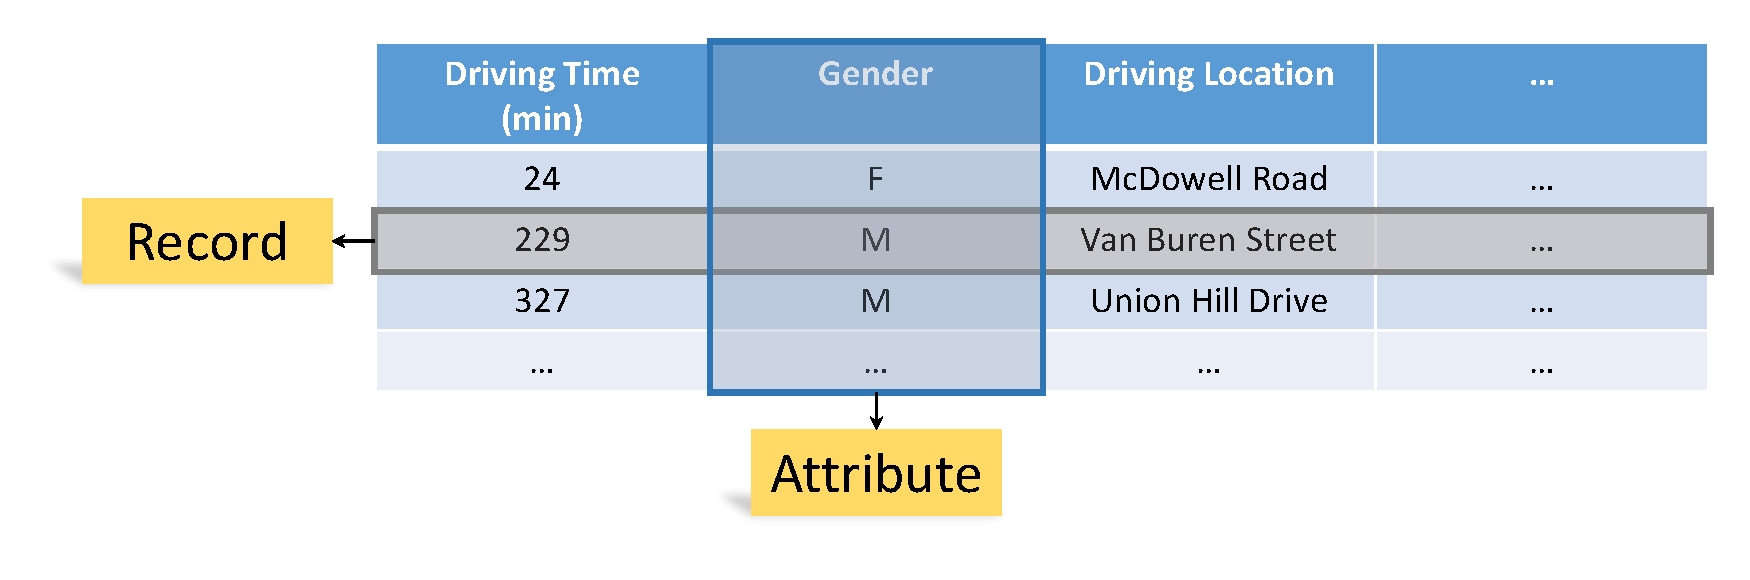
\includegraphics[width=0.9\textwidth]{chapter3/attr_pre}
  %\noindent\rule[0.25\baselineskip]{0.4855\textwidth}{0.95pt}
  \bicaption[fig:attr_pre]{的士司机行车记录数据集}{的士司机行车记录数据集}{Fig}{An illustration of taxi drivers' driving dataset}
\end{figure}

在图\ref{fig:attr_pre}中,我们可以看到该数据集有许多的属性,比如行车时间、司机性别以及行驶地点等等。这些属性的值可以是数值型的,也可以是文字性的。如果数据卖家想基于这些数据的信息量给这个数据集定价,那么其首要问题是弄起初这个数据集含有多少的信息量。因此,我们首要目标是去找到一个合适的方法精确度量该数据集所含有的信息量。在得到了该数据集的信息量之后,我们需要将其映射到一个合适的价格。

用更加形式化的方式叙述上述问题,对于一个有着$m$个属性和$n$条记录的数据集$\bm{D}$,它能表示成一个矩阵$\bm{X}$:
\begin{equation}
\bm{X}=
\left(
\begin{matrix}
 x_{11}      &  x_{12}      & \cdots &  x_{1m}      \\
 x_{21}     &  x_{22}      & \cdots &  x_{2m}      \\
 \vdots & \vdots & \ddots & \vdots \\
  x_{n1}      &  x_{n2}      & \cdots &  x_{nm}      \\
\end{matrix}
\right).
\end{equation}

在矩阵$\bm{X}$中,行向量$\bm{r_i}$表示原数据集中一条记录:
\begin{equation}
\bm{r_i}=\left(
\begin{matrix}
 x_{i1},      &x_{i2},      &\cdots, &x_{im}      \\
\end{matrix}
\right),
\end{equation}

其中,$i=1,...,n$。令$\bm{R}$表示一组记录$\{\bm{r_{i_1}},\bm{r_{i_2}},...,\bm{r_{i_k}}\}$的集合。类似的,列向量$\bm{c_j^\mathrm{T}}$表示原数据集中的一列属性:
\begin{equation}
 \bm{c_j^\mathrm{T}}=\left(
\begin{matrix}
 x_{1j};     &x_{2j};      &\cdots; &x_{nj}      \\
\end{matrix}
\right),
\end{equation}

其中,$j=1,...,m$。同样地,令$\bm{C}$表示一组属性$\{\bm{c_{j_1}},\bm{c_{j_2}},...,\bm{c_{j_k}}\}$的集合。需要指出的是,$\bm{r_i}$中的每个元素的值可以是不同类型的,比如数值、文字、日期等。但是$\bm{c_j}$的元素的值必须是同一类型的。

那么基于信息量的给数据集$\bm{D}$定价的方法可以分为两步:1)量化地度量数据集$\bm{D}$或其子集的信息量$H$;2)基于度量结果,找到一个合适的函数$l(\dot)$,将信息量$H$映射到一个价格$pr$,即$pr=l(H(\bm{D}))$。

为了达到上述目标,在下文中我们首先提出一个基于信息熵的信息量检测方法。然后基于检测结果,我们给出一个定价模型。

\subsection{数据商品信息量的测量}
在本小节中,我们先定义了元组和元组集合。然后,我们基于信息熵\cite{shannon2001mathematical}给出了相应的信息测量方法。

\begin{defn}[元组]
 对于给定的一个数据集$\bm{D}$,元组$\bm{t}$被定义为$\bm{D}$中一条记录$\bm{r}$的非空子集,即$\bm{t} \subseteq \bm{r}$且$\bm{t} \ne \emptyset$。
\end{defn}

\begin{defn}[元组集合]
元组集合$Tup$是一系列元组$\{\bm{t_{i_1}},\bm{t_{i_2}},...,\bm{t_{i_k}}\}$的集合。因此,$Tup$也是数据集$\bm{D}$的非空子集,即$Tup \subseteq \bm{D}$ 且 $Tup \ne \emptyset$。
\label{def:tuple_set}
\end{defn}

对于定义\ref{def:tuple_set},元组集合$Tup$可以是数据集的子集也可以就是数据集本身。实际上,元组集合是本文提出信息测量方法的最小单元。以下四个信息熵测量指标都是基于元组的。

\begin{defn}[数据信息熵]
对于一个有着$n$条元组$\{\bm{t_i}$$|i=1,...,n\}$的元组集合$Tup$,其数据信息熵$H_{ind}$定义为:
\begin{equation}
  H_{ind}(Tup)=-\sum_{\bm{t_i} \in Tup}p(\bm{t_i})\log_{b}p(\bm{t_i}),
  \label{eq:data_individual_entropy}
\end{equation}
\label{def:data_individual_entropy}
\end{defn}
其中,$b$是公式\ref{eq:data_individual_entropy}中对数的基。信息常用度量单位为比特,当对数基底$b$取为$2$时。除非特别指出,下文所有的对数都指的是以$2$为基底的对数,即$\log_2x$。数据信息熵是本文提出数据信息测量方法的最基础概念,它能测量出单个元组集合的信息量。

\begin{defn}[数据联合熵]

对于有$n_1$条元组的元组集合$Tup_1$和有$n_2$条元组的元组集合$Tup_2$,它们的数据联合熵$H_{joint}$定义为:

\begin{equation}\label{eq:joint_entropy}
  \begin{aligned}
    H_{joint}(Tup_1,Tup_2)=-\sum_{\bm{t_i} \in Tup_1} \sum_{\bm{t_j} \in Tup_2} p(\bm{t_i},\bm{t_j}) \log p(\bm{t_i},\bm{t_j})。
  \end{aligned}
\end{equation}

\label{def:data_joint_entropy}
\end{defn}

需要指出的是数据联合熵是可以轻易地扩展到多个元组集合的信息测量。

\begin{defn}[数据条件熵]
对于有$n_1$条元组的元组集合$Tup_1$和有$n_2$条元组的元组集合$Tup_2$,那么在已知$Tup_1$的条件下$Tup_2$的信息熵被定义为
\begin{equation}\label{eq:conditional_entropy}
  \begin{aligned}
    H_{cond}(Tup_2|Tup_1)=-\sum_{\bm{t_i} \in Tup_1} \sum_{\bm{t_j} \in Tup_2} p(\bm{t_i},\bm{t_j})\log p(\bm{t_j}|\bm{t_i}),
  \end{aligned}
\end{equation}
\label{def:data_conditional_entropy}
\end{defn}
其中$H_{cond}(Tup_2|Tup_1)=0$,当且仅当$Tup_2$被$Tup_1$完全决定。换句话说,一旦$Tup_1$已知,$Tup_2$就被唯一确定了。相反的情况是,$H_{cond}(Tup_2|Tup_1)=H_{ind}(Tup_2)$当且仅当$H_{ind}(Tup_1)$和$H_{ind}(Tup_2)$是统计独立的,换句话说就是即使$Tup_1$已知,也不能获得$Tup_2$的任何信息。

\begin{defn}[数据互信息]
对于有$n_1$条元组的元组集合$Tup_1$和有$n_2$条元组的元组集合$Tup_2$,$Tup_1$和$Tup_2$的数据互信息$I$定义为:

\begin{equation}
\label{eq:mutual_information}
  \begin{aligned}
    I(Tup_1;Tup_2)=\sum_{\bm{t_i} \in Tup_1} \sum_{\bm{t_j} \in Tup_2} p(\bm{t_i},\bm{t_j}) \log\frac{p(\bm{t_i},\bm{t_j})}{p(\bm{t_i})p(\bm{t_j})}。
  \end{aligned}
\end{equation}

\label{def:data_mutal_information}
\end{defn}


相比于数据条件熵,数据互信息是被用来度量两个元组的依赖程度。

需要指出的是,元组的元素也可以是连续型数值的。然而上述定义的相关熵都是默认元组元素是离散的。以上定义可以通过将求和符号替换为积分符号后扩展到连续型元组上:

\begin{equation}
  H_{ind}(Tup)=-\int_{\bm{t_i} \in Tup}p(\bm{t_i})\log p(\bm{t_i}),
\end{equation}
\begin{equation}
  H_{joint}(Tup_1,Tup_2)=-\int_{\bm{t_i} \in Tup_1} \int_{\bm{t_j} \in Tup_2} p(\bm{t_i},\bm{t_j}) \log p(\bm{t_i},\bm{t_j}),
\end{equation}
\begin{equation}
  H_{cond}(Tup_2|Tup_1)=-\int_{\bm{t_i} \in Tup_1} \int_{\bm{t_j} \in Tup_2} p(\bm{t_i},\bm{t_j})\log p(\bm{t_j}|\bm{t_i}),
\end{equation}
\begin{equation}
  I(Tup_1;Tup_2)=\int_{\bm{t_i} \in Tup_1} \int_{\bm{t_j} \in Tup_2} p(\bm{t_i},\bm{t_j}) \log\frac{p(\bm{t_i},\bm{t_j})}{p(\bm{t_i})p(\bm{t_j})}.
\end{equation}

然而,对于连续型变量而言,通常是很难确定其概率密度函数。另一方面,在计算机中积分的数值计算也是存在误差的。因此,计算连续型数据的数据信息熵的一般方法是将连续的输入空间切分为若干个离散的子空间,然后按照离散型变量计算其信息熵然。然而这种方法的内部误差会降低计算最后的熵的精确度,那么这就会影响定价策略。对于那些连续型、离散型数据均有的元组,其相应数据信息熵的计算方法是我们未来的工作之一。

此外,\cite{shannon2001mathematical}还列出一系列熵的性质,后续定价函数的讨论涉及到这些性质,因此我们简单陈述下相关性质。

\begin{propt}[数据信息熵的非负性]
\label{pr:entropry_non_negativity}
给定两个元组集合$Tup_1$和$Tup_2$,我们有

\begin{equation}
  H_{ind}(Tup_1)\ge 0, H_{ind}(Tup_2)\ge 0,
\end{equation}
\begin{equation}
  H_{joint}(Tup_1,Tup_2)\ge 0,
\end{equation}
\begin{equation}
  H_{cond}(Tup_1|Tup_2)\ge 0, H_{cond}(Tup_2|Tup_1)\ge 0,
\end{equation}
\begin{equation}
  I(Tup_1;Tup_2)\ge 0.
\end{equation}


性质\ref{pr:entropry_non_negativity}的证明如下:
\begin{proof}
首先来关注数据信息熵,$H_{ind}(Tup)$,其定义如下:

\begin{equation}
    H_{ind}(Tup)=-\sum_{\bm{t_i} \in Tup}p(\bm{t_i})\log p(\bm{t_i})。
    \label{proof:individual_entropy}
\end{equation}

由于 $0\le p(\bm{t_i}) \le 1$,那么

\begin{equation}
\log p(\bm{t_i}) \le 0。
\end{equation}

因此,根据公式(\ref{proof:individual_entropy}), $H_{ind}(Tup)$ 一定是非负的。

$H_{joint}(\cdot)$,$H_{cond}(\cdot)$, $H_{cond}(\cdot)$以及$I(\cdot)$的非负性同样可以采用上述类似步骤证明。

\end{proof}
\end{propt}

\begin{propt}[不同数据信息熵之间的关系]
给定两个元组集合$Tup_1$和$Tup_2$,我们有

\begin{equation}
\label{pr:entropry_relationships}
  H_{joint}(Tup_1,Tup_2)\le H_{ind}(Tup_1)+H_{ind}(Tup_2),
\end{equation}
\begin{equation}
  H_{joint}(Tup_1,Tup_2)\ge H_{ind}(Tup_1),
\end{equation}
\begin{equation}
  H_{joint}(Tup_1,Tup_2)\ge H_{ind}(Tup_2).
\end{equation}

性质\ref{pr:entropry_relationships}的证明如下:
\begin{proof}


首先从数据互信息的定义入手:

\begin{equation}
    I(Tup_1;Tup_2)=\sum_{\bm{t_i} \in Tup_1} \sum_{\bm{t_j} \in Tup_2} p(\bm{t_i},\bm{t_j}) \log\frac{p(\bm{t_i},\bm{t_j})}{p(\bm{t_i})p(\bm{t_j})}.
    \label{app:mutual_information}
\end{equation}


公式(\ref{app:mutual_information})能被重写为:
\begin{equation}
    \begin{aligned}
    I(Tup_1;Tup_2)&=\sum_{\bm{t_i} \in Tup_1} \sum_{\bm{t_j} \in Tup_2} p(\bm{t_i},\bm{t_j}) [\log p(\bm{t_i},\bm{t_j})\\
    &- \log p(\bm{t_i}) - \log p(\bm{t_j})]\\
    &=\sum_{\bm{t_i} \in Tup_1} \sum_{\bm{t_j} \in Tup_2} p(\bm{t_i},\bm{t_j})\log p(\bm{t_i},\bm{t_j})\\
    &-\sum_{\bm{t_i} \in Tup_1} \sum_{\bm{t_j} \in Tup_2} p(\bm{t_i},\bm{t_j})\log p(\bm{t_i})\\
    &-\sum_{\bm{t_i} \in Tup_1} \sum_{\bm{t_j} \in Tup_2} p(\bm{t_i},\bm{t_j})\log p(\bm{t_j}).
    \end{aligned}
    \label{eq:mutal_information_rewrite1}
\end{equation}

根据定义\ref{def:data_individual_entropy}和定义\ref{def:data_joint_entropy},公式~(\ref{eq:mutal_information_rewrite1}) 能进一步写成:

\begin{equation}
\begin{aligned}
    H_{joint}(Tup_1,Tup_2)&=H_{ind}(Tup_1)+H_{ind}(Tup_2)\\
    &-I(Tup_1;Tup_2).
\label{eq:mutal_information_rewrite2}
\end{aligned}
\end{equation}

由于数据信息熵和数据互信息的非负性,我们有:

\begin{equation}
  H_{joint}(Tup_1,Tup_2)\le H_{ind}(Tup_1)+H_{ind}(Tup_2),
\end{equation}

另一方面,根据定义\ref{def:data_individual_entropy},定义\ref{def:data_joint_entropy},以及定义\ref{def:data_conditional_entropy}, 公式(\ref{eq:mutal_information_rewrite1})能进一步写成:
\begin{equation}
    H_{joint}(Tup_1,Tup_2)=H_{cond}(Tup_1|Tup_2)+H_{ind}(Tup_2),
\end{equation}
\begin{equation}
    H_{joint}(Tup_1,Tup_2)=H_{cond}(Tup_2|Tup_1)+H_{ind}(Tup_1).
\end{equation}

类似地,由于数据信息熵的非负性,那么有:

\begin{equation}
  H_{joint}(Tup_1,Tup_2)\ge H_{ind}(Tup_1),
\end{equation}
\begin{equation}
  H_{joint}(Tup_1,Tup_2)\ge H_{ind}(Tup_2).
\end{equation}

\end{proof}
\end{propt}


\subsection{通用定价模型}

在本小节中,我们提出了一个基于数据信息熵的通用定价模型,而不是给出一个具体的定价函数。此外,该定价模型的相关性质和优点在本小节中也会进行讨论。

\begin{defn}[定价函数]
对一个给定的数据集$\bm{D}$,定价函数${pr(\bm{D})}:\bm{D}\to \mathbb{R^{+}}$, 其中 $\mathbb{R^{+}}$ 非负实数。一个基于数据信息熵的定价函数是:
\begin{equation}
  pr(\cdot) \equiv l(H(\cdot)),
  \label{eq:pricing_function}
\end{equation}
其中$l(\cdot)$ 是一个非递减的联系函数,它应该满足如下条件:
\begin{equation}
\forall x_1 \ge x_2, l(x_1) \ge l(x_2),
\label{eq:link_function_property1}
\end{equation}
\begin{equation}
\forall x_1, x_2 \ge 0, l(x_1+x_2) \le l(x_1)+l(x_2).
\label{eq:link_function_property2}
\end{equation}
\end{defn}

\begin{exmp}
对于两个数据集$\bm{D_1}$和$\bm{D_2}$以及一个基于数据信息熵的定价函数$pr(\cdot) \equiv l(H(\cdot))$,如果$H(\bm{D_1})\ge H(\bm{D_2})$,那么有$pr(\bm{D_1})\ge pr(\bm{D_2})$。
\end{exmp}

为了陈述简洁,上述数据信息熵的定价函数都指的是数据独立信息熵或者数据联合熵,取决于$H(\cdot)$中参数个数。选择具体的定价函数要取决于具体的市场情况,这也是本文的未来工作之一。

\begin{propt}[定价函数的非负性]
定价函数的输出一定是大于零的,即$pr(\cdot) \ge 0$总是成立。
\label{pr:pricing_function_pr_1}
\end{propt}

定价函数的非负性是显然的,因为数据卖家在出售商品的同时还倒贴钱给数据买家。接下来,基于数据信息熵的定价函数的\textit{无套利}性质会被讨论,这个性质也是其最大的优点。为了详细地讨论这个性质,我们首先要介绍下一个数据集中的操作,即\textit{连接}。

\begin{defn}[数据集连接]

给定两个数据集$\bm{D_1}$和$\bm{D_2}$,$\bm{D_1}$有$n_1$条记录$\bm{R_1}$和$m_1$条属性$\bm{C_1}$,$\bm{D_2}$有$n_2$条记录$\bm{R_2}$和$m_2$条属性$\bm{C_2}$,$\bm{D_1}$和$\bm{D_2}$的连接$\bm{D_J}$定义为:

\begin{equation}
\bm{D_J}=\bm{D_1} \circledcirc \bm{D_2}.
\end{equation}
\end{defn}

这里给出数据连接操作的两个例子:

\begin{case}
如果在数据集$\bm{D_1}$和$\bm{D_2}$中没有共同的属性,即$\bm{C_1} \cap \bm{C_2} = \emptyset$,那么它们的连接$\bm{D_J}$就会有$n_1+n_2$条记录和$m_1+m_2$条属性。

\end{case}

\begin{case}
如果在数据集$\bm{D_1}$和$\bm{D_2}$中有共同的属性,即$\bm{C_1} \cap \bm{C_2} \ne \emptyset$,那么它们的连接$\bm{D_J}$就会有$n_1+n_2$条记录和$\|\bm{C_1} \cup \bm{C_2}\|$ 条属性。

\end{case}

数据集\textit{连接}的操作能被扩展到多个数据集的情况。如果有多个数据集 $\bm{D_1,D_2,...,D_k}$,我们把他们的连接集合记为$\bm{D_J}=\circledcirc_{i=1}^k \bm{D_i}$。值得注意的是这里的连接操作不同于SQL类的数据库连接操作。为了更加直观地说明这个连接操作,我们举出了如下例子:

\begin{exmp}
数据集$\bm{D_1}$有$3$条记录和$3$个属性$\{a,b,c\}$,数据集$\bm{D_2}$有$4$条记录和$2$个属性$\{c,d\}$。它们的连接数据集$\bm{D_1} \circledcirc \bm{D_2}$将会有$7$条记录和$4$个属性$\{a,b,c,d\}$,如图\ref{fig:joint_data_set}所示。在连接数据集中,那些非共同属性的缺失值是用'\#'填满。
\end{exmp}

\begin{figure}[h]
  \centering
    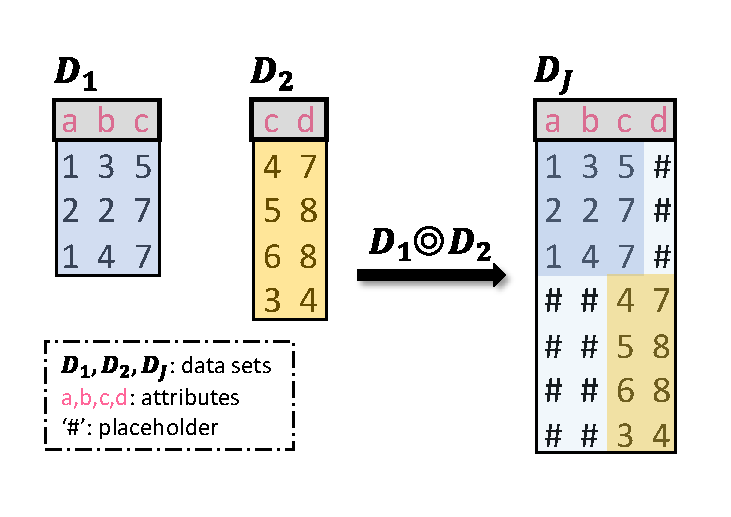
\includegraphics[width=0.7\textwidth]{chapter3/joint_data_set}
  %\noindent\rule[0.25\baselineskip]{0.4855\textwidth}{0.95pt}
  \bicaption[fig:joint_data_set]{数据集连接操作示意图}{数据集连接操作示意图}{Fig}{An illustration of dataset join}
\end{figure}

\begin{propt}[定价函数的无套利性]
对于数据集$\bm{D_1}$和$\bm{D_2}$,如果$\bm{D_1} \circledcirc \bm{D_2}$的价格小于或等于$\bm{D_1}$和$\bm{D_2}$的简单求和,那么定价函数就是无套利的,即:
\begin{equation}
  \begin{aligned}
  pr(\bm{D_1} \circledcirc \bm{D_2}) \le pr(\bm{D_1})+pr(\bm{D_2}).
  \end{aligned}
\end{equation}
\label{pr:arbitrage-free}
\end{propt}

在经济学和金融学中,套利指的是通过不同市场之间的价格差异获得利润差的行为。具体说来就是套利者可以通过在某个市场低价购入物品,然后在另一个市场高价卖出该物品。然而,这个概念在金融市场和数据市场是有些许差异的。现在假设有三个数据集$\bm{D_1}$,$\bm{D_2}$和$\bm{D_3}$,相应的价格分别为$p_1$, $p_2$, and $p_3$,如果数据集$\bm{D_3}$可以通过连接$\bm{D_1}$和$\bm{D_2}$得到,即$\bm{D_3}=\bm{D_1} \circledcirc \bm{D_2}$。当$p_3\ge p_1+p_2$,套利的条件就产生了。一个精明的数据消$p_3$费者可以通过分别购买数据集$\bm{D_1}$和$\bm{D_2}$以一个相对原价$p_3$更低的价格$p_1+p_2$获得数据集$\bm{D_3}$。因此,一个好的定价函数应当是能避免套利行为的。

\begin{lem}
对于定价函数$pr(\cdot) \equiv l(H(\cdot))$,这里$l(\cdot)$是一个非递减的联系函数。如果$l(\cdot)$满足公式(\ref{eq:link_function_property1})和公式(\ref{eq:link_function_property2}),那么$pr(\cdot)$是无套利的。
\label{lemma:arbitrage-free}

\begin{proof}

给定两个数据集$\bm{D_1}$和$\bm{D_2}$,以及一个定价函数$pr(\cdot)$,$pr(\cdot) \equiv l(H(\cdot))$, 其中$l(\cdot)$是非递减的联系函数。

根据性质~\ref{pr:entropry_relationships}, $H(\bm{D_1})$, $H(\bm{D_2})$和$H(\bm{D_1},\bm{D_2})$的关系如下:

\begin{equation}
  H(\bm{D_1},\bm{D_2})\le H(\bm{D_1})+H(\bm{D_2}),
\end{equation}
\begin{equation}
  H(\bm{D_1},\bm{D_2})\ge H(\bm{D_1}),
\end{equation}
\begin{equation}
  H(\bm{D_1},\bm{D_2})\ge H(\bm{D_2}).
\end{equation}


因为$pr(\cdot) \equiv l(H(\cdot))$和$l(\cdot)$满足公式~(\ref{eq:link_function_property1})和公式(\ref{eq:link_function_property2}),所以我们有:

\begin{equation}
  pr(\bm{D_1}\circledcirc \bm{D_2})\le pr(\bm{D_1})+pr(\bm{D_2}),
\end{equation}
\begin{equation}
  pr(\bm{D_1}\circledcirc \bm{D_2})\ge pr(\bm{D_1}),
\end{equation}
\begin{equation}
  pr(\bm{D_1}\circledcirc \bm{D_2})\ge pr(\bm{D_2}).
\end{equation}

因此,定价函数$pr(\cdot)$是无套利的。

\end{proof}

\end{lem}

无套利的性质是基于数据信息熵的定价函数最好的一个性质,这也是之前很多研究\cite{koutris2012querymarket,koutris2015query,lin2014arbitrage}所追求的目标。

\subsection{讨论}

理论上,我们提出的信息量测量方法能被应用到任何类型的数据。但是,实际中只有全离散型或者全连续型能被精确地度量。因为在这种情形下,是相对容易去找到其概率密度函数的。测量混合型数据的信息量是我们未来的工作之一。

关于本小节中提出的基于数据信息熵定价函数,其最大的优点就是其无套利性质。之前的一些基于查询的数据定价的研究\cite{balazinska2011data,koutris2012querymarket,koutris2015query}都是致力于使他们提出的定价函数变成无套利的。论文\cite{balazinska2011data}提出了基于查询的数据定价的原型,在该文中一个关于在线数据市场如何计算查询价格的简单例子被提出来了。尽管后续的研究者基于论文\cite{balazinska2011data}提出了不同的定价函数,但是他们仍然没有解决如何为查询的最小单元(视图)定价的问题,这些最小单元的定价仍然是主观定价的。我们提出的数据定价指标——数据信息熵,也许能提供一个新的视角去解决论文\cite{balazinska2011data,koutris2012querymarket,koutris2015query}所遗留的问题。因为数据信息熵能够为数据定价者提供不同视图之间的明确的定价关系,以避免套利行为的发生。


\section{实验与评估}
\label{sec:evaluation}
为了推动数据市场的经营者采用本文提出的数据信息熵来指导他们的商品定价,我们首先需要验证提出的数据定价指标的合理性和有效性。我们从两个方面评估数据信息熵:1)数据集数据信息熵和该数据集大小的关系。根据大量数据交易记录,一个数据集的信息量大小一般是与该数据集的大小成正比。如果数据信息熵能度量一个数据集的信息量,那么它首先应是数据集大小的非递减函数;2)数据集的数据信息熵和和在该数据集上分类器正确率的的关系。根据大量机器学习实验的经验,经过一个数据集训练的分类器的分类正确率是与该数据集的有效信息量是有关的。具体一点地说,如果有更多的有效信息被分类器学到了,那么该分类器之后的分类正确率就会更高。那么这意味着,如果数据信息熵能度量出数据集的有效信息量,其应当与该数据集上的分类器的分类正确率成正比。

为了研究上述两个关系,我们按照以下流程设计了实验步骤:1)对于一个给定的数据集,我们先将其按照记录数或者不同的属性数将其切分成若干个元组集合;2)测量这些元组集合的数据信息熵;3)在这些元组集合上训练不同的分类器,并记录相应的分类正确率。上述这些实验是在六个公开的研究数据集和一个大规模电信工业数据集上做的。

\subsection{实践中遇到的问题}

\subsubsection{基于Parzen窗口函数的概率密度估计}
\label{subsubsec:parzen_window}

前面提到过对于离散型数据的数据信息熵计算是很容易的,但是对于连续型数据集就比较难了,因为连续型数据的概率密度函数是不好估计的。这里,我们采用了基于Parzen窗口函数的概率密度估计来计算连续型数据的数据信息熵。下面,就简单地介绍下基于Parzen窗口函数的概率密度估计方法。

在实际中,数据集的样本数总是有限的。这造成的结果就是我们通常很难用这些有限的样本数计算连续空间中的积分。比较常用的解决方案就是将连续数据空间划分为若干个离散的空间,然后在这些离散空间中求和积分。但是这种离散化求积分的方法是不足够精确的。另一个解决方案就是利用基于Parzen窗口函数\cite{parzen1962estimation}的概率密度估计方法来估计概率密度函数,从而去计算数据信息熵。

对于连续型随机变量$x$的$n$个采样样本$x_1, x_2, ..., x_n$,如果其真正的概率密度函数是$p(\mathit{x})$,那么它的估计的概率密度函数$\hat{p}(\mathit{x})$被定义为:

\begin{equation}
  \begin{aligned}
    \hat{p}(x)=\frac{1}{n}\sum_{i=1}^{n}\phi(x-x_i,h),
  \end{aligned}
\end{equation}
其中$\phi(\cdot)$是Parzen窗口函数,$h$是窗口宽度。Parzen\cite{parzen1962estimation}已经证明了如果选择了合适的窗口函数$\phi(\cdot)$和窗口宽度$h$,且样本数$n$趋向于无穷时,那么估计的概率密度函数$\hat{p}(\mathit{x})$是可以收敛到真正的概率密度函数$p(\mathit{x})$的。

但窗口函数的选择还是有限制的,其中就要求其必须是有限且非负:

\begin{equation}
  \begin{aligned}
    \int \phi(y,h)dy = 1,
  \end{aligned}
\end{equation}
其中窗口宽度$h$必须是样本数$n$的函数,且满足:

\begin{equation}
  \begin{aligned}
    \lim_{n\rightarrow \infty} h(n)=0.
  \end{aligned}
\end{equation}

高斯和矩形函数是最常用的窗口函数。在本文中,我们采用高斯函数作为窗口函数:

\begin{equation}
  \begin{aligned}
    \phi(z,h)=\frac{1}{(2\pi)^{d/2}h^d\|\sigma\|^{1/2}}\exp(-\frac{z^T\sigma^{-1}z}{2h^2}),
  \end{aligned}
\end{equation}
其中$\sigma$表示$d$维随机向量$z$的协方差矩阵。

我们利用基于Parzen窗口函数的概率密度估计方法来计算连续型数据的数据信息熵。

\subsubsection{多个分类器}

为了验证我们提出的信息量测量指标和方法的通用性,我们在不同数据集上训练了不同分类器。这些分类器都是目前机器学习领域最常用也是被研究地最透彻的分类器,比如支持向量机(Support Vector Machine, SVM),决策树(Decision Tree, DT)以及线性判别分析(Linear Discriminative Analysis, LDA)。

支持向量机\cite{burges1998tutorial,vapnik2013nature,milenova2005svm}在高维或无限维空间中构造超平面或超平面集合,如图\ref{fig:svm},其可以用于分类、回归或其他任务。直观来说,分类边界距离最近的训练样本点越远越好,因为这样可以减小支持向量的泛化误差。

\begin{figure}[h]
  \centering
    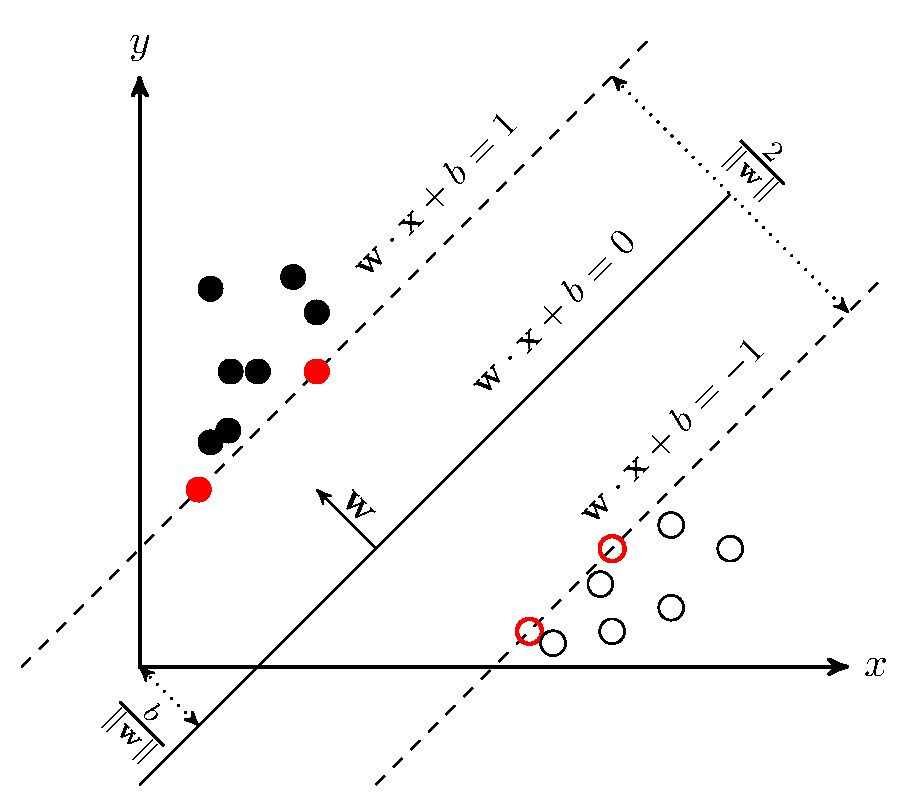
\includegraphics[width=0.6\textwidth]{chapter3/svm}
  %\noindent\rule[0.25\baselineskip]{0.4855\textwidth}{0.95pt}
  \bicaption[fig:svm]{支持向量机示意图}{支持向量机示意图}{Fig}{An illustration of support vector machine}
\end{figure}

决策树\cite{safavian1990survey,hu2015differential} 是一个预测模型;它代表的是对象属性与对象值之间的一种函数关系。树中每个节点表示某个对象,而每条边则代表某个可能的属性值,而每个叶节点则对应从根节点到该叶节点所经历的路径所表示的对象的值,如图\ref{fig:dt}。决策树仅有单一输出。数据挖掘中决策树是一种经常要用到的技术,可以用于分析数据,同样也可以用来作预测。

\begin{figure}[h]
  \centering
    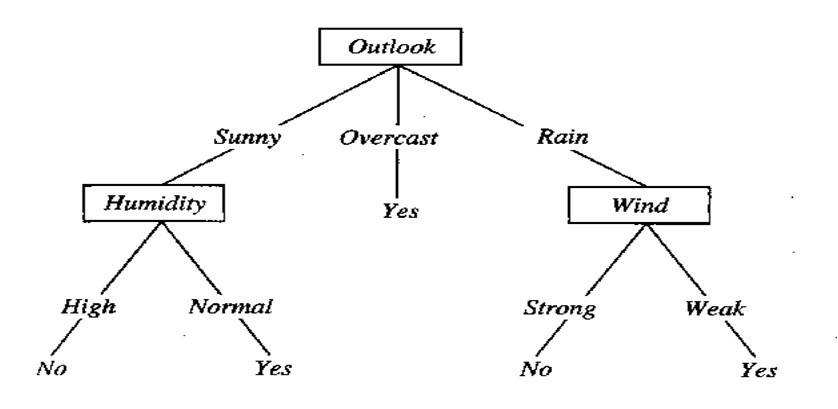
\includegraphics[width=0.6\textwidth]{chapter3/dt}
  %\noindent\rule[0.25\baselineskip]{0.4855\textwidth}{0.95pt}
  \bicaption[fig:dt]{决策树示意图}{决策树示意图}{Fig}{An illustration of decision tree}
\end{figure}

线性判别分析\cite{webb2003statistical}是最早被提出的分类器之一,它能在输入空间中学到线性分类边界,如图\ref{fig:lda}。线性判别分析能用来做二分类或者多分类的问题。

\begin{figure}[h]
  \centering
    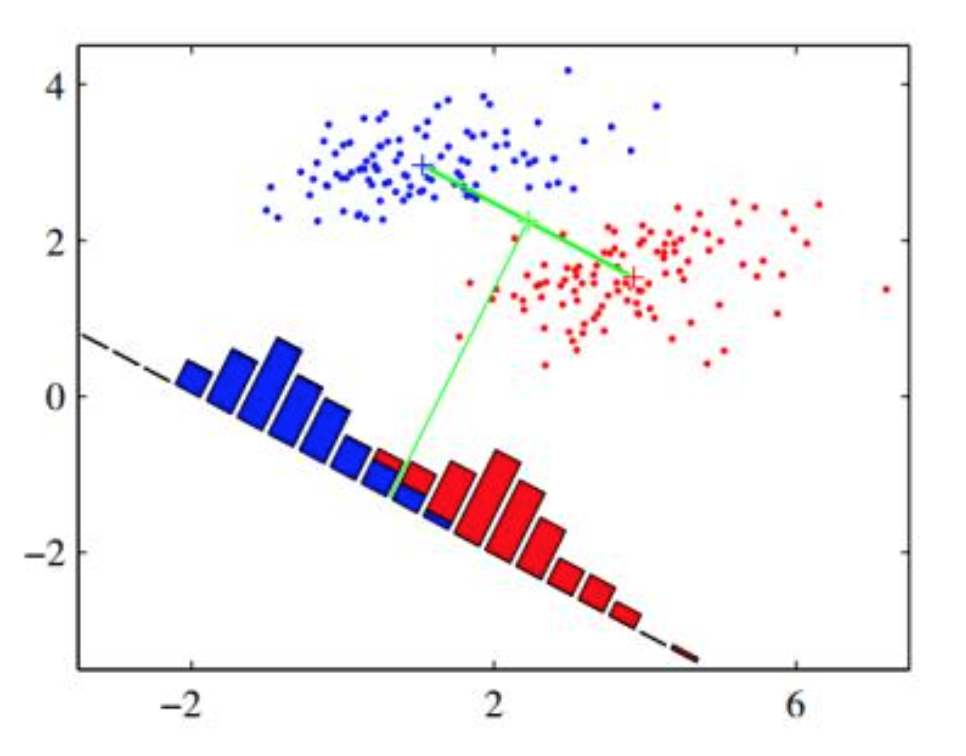
\includegraphics[width=0.6\textwidth]{chapter3/lda}
  %\noindent\rule[0.25\baselineskip]{0.4855\textwidth}{0.95pt}
  \bicaption[fig:lda]{线性判别分析示意图}{线性判别分析示意图}{Fig}{An illustration of linear discriminative analysis}
\end{figure}

\subsection{在公开研究数据集上的实验}

\subsubsection{UCI数据集}

我们所做的实验都是基于UCI机器学习公开数据集\cite{Lichman:2013},这些数据集都是有类标签的。我们把这些数据集的详细信息总结在表\ref{tab:datasets_used}。

\begin{table*}[!t]
\centering
\bicaption[tab:datasets_used]{实验中用到的UCI数据集}{实验中用到的UCI数据集}{Table}{UCI Datasets Used in The Experiments}
\begin{tabular}{|c|c|c|c|c|c|c|}
\hline
数据集名称 &Letter &Mushroom &Nursery &Ecoli &Ionosphere &Vehicle \\
\hline
\hline
缩写 &LET &MUS &NUR &ECO &ION &VEH\\
\hline
原始数据类型 &
\multicolumn{3}{c|}{离散型}&
\multicolumn{3}{c|}{连续型}\\
\hline
预处理方法 &
\multicolumn{3}{c|}{---}&
\multicolumn{3}{c|}{z-score ($\mu=0,\sigma=1$)}\\
\hline
记录数 &$20000$ &$8124$ &$12960$ &$336$ &$351$ &$946$ \\
\hline
属性数 &$16$ &$22$ &$8$ &$7$ &$34$ &$18$\\
\hline
种类数 &$26$ &$2$ &$4$ &$8$ &$2$ &$4$\\
\hline
测试方法&
\multicolumn{3}{c|}{10折交叉验证法}&
\multicolumn{2}{c|}{留一法}&
10折交叉验证法\\
\hline
来源&
\multicolumn{6}{c|}{UCI机器学习数据库~\cite{Lichman:2013}}\\
\hline
\end{tabular}
\end{table*}

具体来说,前三个数据集LET,MUS和NUR是离散型数据集。后三个数据集ECO,ION和VEH是连续型数据集。连续型数据中的属性值经过了预处理使得其服从均值为零,单位方差的正态分布。

数据集LET包含了$20000$个大写字母的初始数值属性,其总共分为$26$类,也就是$26$个英文字母。属性值是在$0$到$15$变化的整数。我们在该数据集上利用10折交叉验证法测试训练的分类器。

数据集MUS包含$23$种蘑菇的$22$条属性的$8124$条记录,这些记录总共分为两类,即有毒的蘑菇和无毒的蘑菇。我们在这个数据集上仍采用10折交叉验证法。

数据集NUR总共有$8$个属性的$12960$条离散数据记录,共分成$4$类。我们在这个数据集上仍采用10折交叉验证法。

数据集ECO包含$7$条属性的$336$条记录,共分成$8$类。因为该数据集包含的记录很少,我们在该数据集上使用是的留一交叉验证法。

数据集ION包含$34$个属性的$351$记录,共分成两类。在这个数据集上,我们仍然采用留一检查验证法。

最后一个数据集ION包含$18$个属性的$946$条记录,共分成$4$个状态。在该数据集上,我们仍然采用10折交叉验证法。

上述列出的这些数据集在记录数、属性数以及数据类型上都有所不同。我们之所以在这么多不同的数据集上训练了不同的分类器,是希望能做一个完成的测试,以此来验证我们提出ed数据定价指标的合理性。

\subsubsection{两种数据集切割方式}
\label{subsubsec:two_splitting_ways}

正如前面\ref{sec:data pricing strategy}小节讨论的,数据市场上的买家往往只会购买完整数据集的部分子集。具体来说就是,他们更倾向于购买完整数据集的部分记录或者部分属性。为了更好地拟合买家的市场行为,对于一个给定的数据集,我们按照如下两种划分方式进行实验:1)按照数据集的属性划分;2)按照数据集的记录划分。这两种划分方式可以参照图\ref{fig:split_dataset}。在将给定数据集划分成不同的元组集合后,我们就分别测量这些元组集合的数据信息熵,再测量三个分类器在它们上面的分类正确率。

\begin{figure}[h]
  \centering
    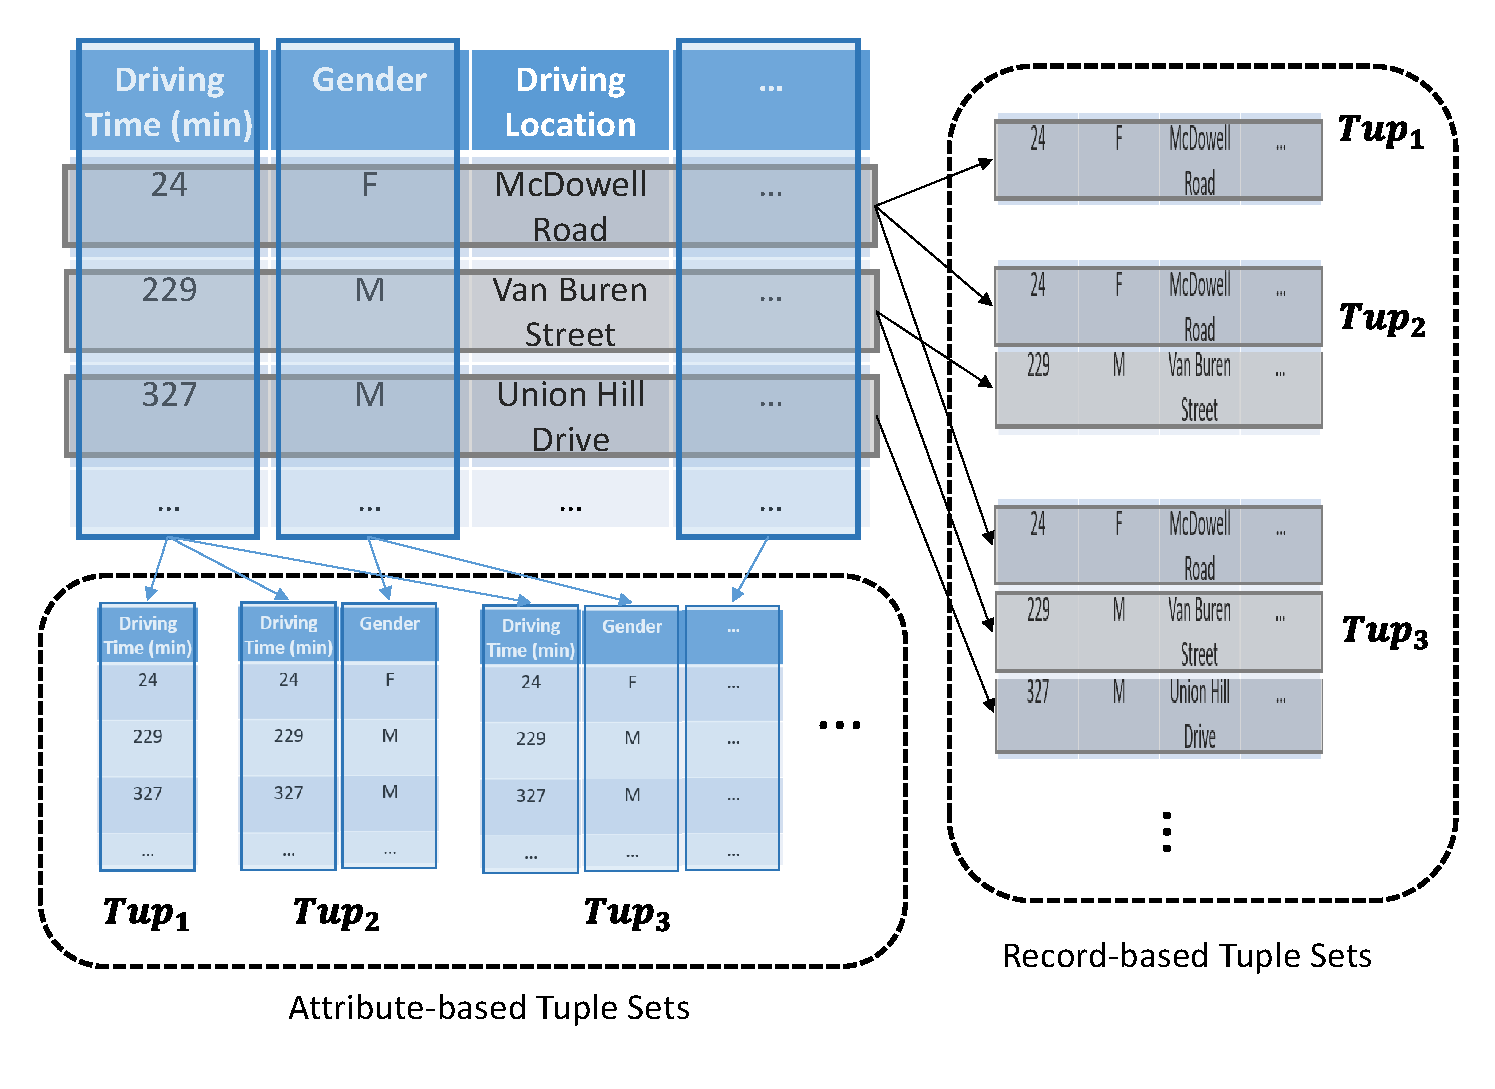
\includegraphics[width=0.7\textwidth]{chapter3/split_dataset}
  %\noindent\rule[0.25\baselineskip]{0.4855\textwidth}{0.95pt}
  \bicaption[fig:split_dataset]{数据集的两种切分方式}{数据集的两种切分方式}{Fig}{Two ways for splitting a datase into tuple sets}
\end{figure}

\subsubsection{基于属性划分的元组集合的实验}
在该实验中,对于一个给定的数据集,我们根据其属性将其划分成含不同属性数的元组集合。然后我们测量这些元组集合的数据信息熵。紧接着,我们基于这些元组集合训练三个分类器,然后记录这三个分类器在这些元组集合上的分类正确率。

例如,数据集ECO总共有七个属性。我们首先将其切分成七个不同的元组集合,这些元组集合分别包含原始数据集ECO的1,2,3,4,5,6,7个属性。然后,我们利用本文提出的数据信息熵来度量这些元组集合的信息量。紧接着,再基于这七个元组集合分别训练支持向量机、决策树和线性判别分析三种分类器,记录下这三个分类器在相应元组集合的分类正确率。剩下的数据集也采用上述同样的步骤进行实验。该实验相关的所有结果被绘制在图\ref{fig:exp2_1},\ref{fig:exp2_2}和\ref{fig:exp2_3}中。

\begin{figure}[h]
	\centering
	\subfigure[ecoli]{
		\label{fig:ecoli_exp2}
		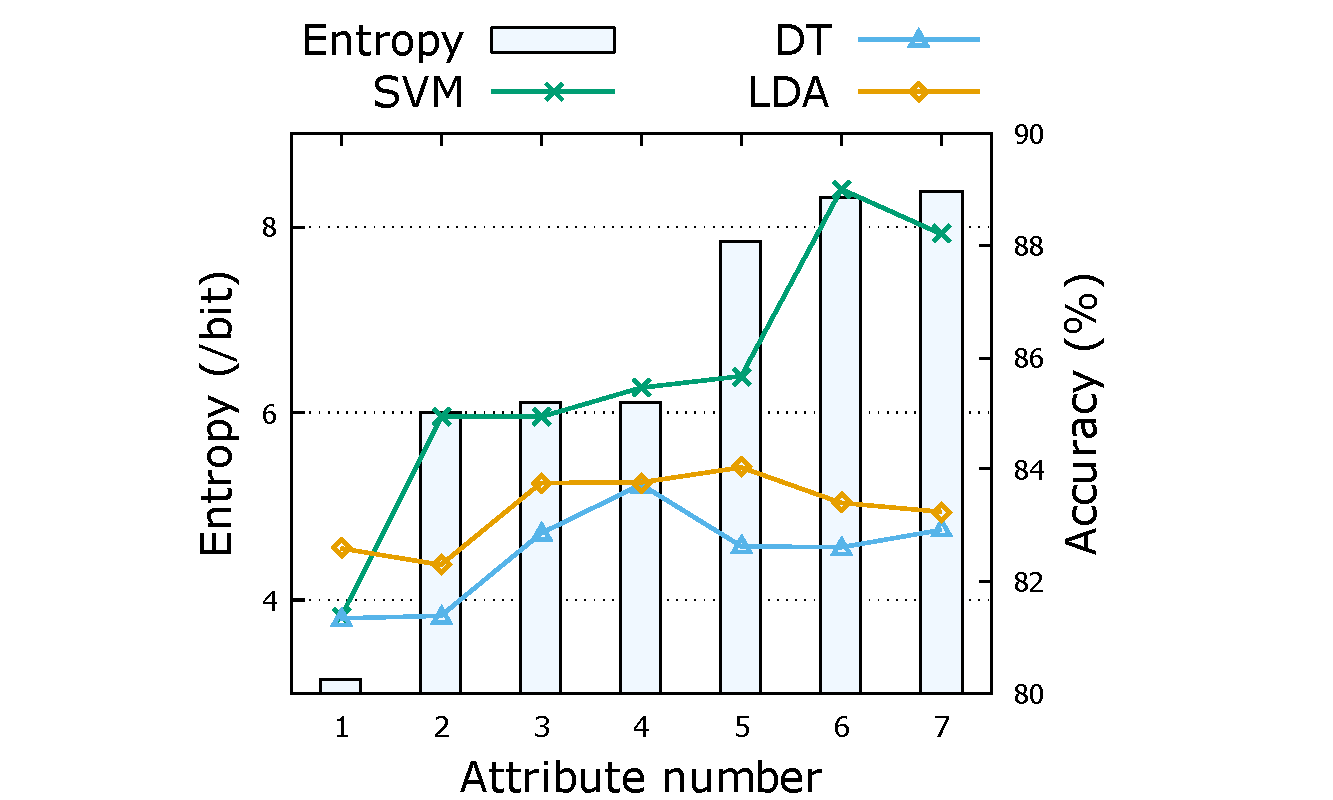
\includegraphics[width=0.6\textwidth]{chapter3/ecoli_experiment_2_with_3_classifiers}
	}
	\subfigure[ionosphere]{
		\label{fig:ionosphere_exp2}
		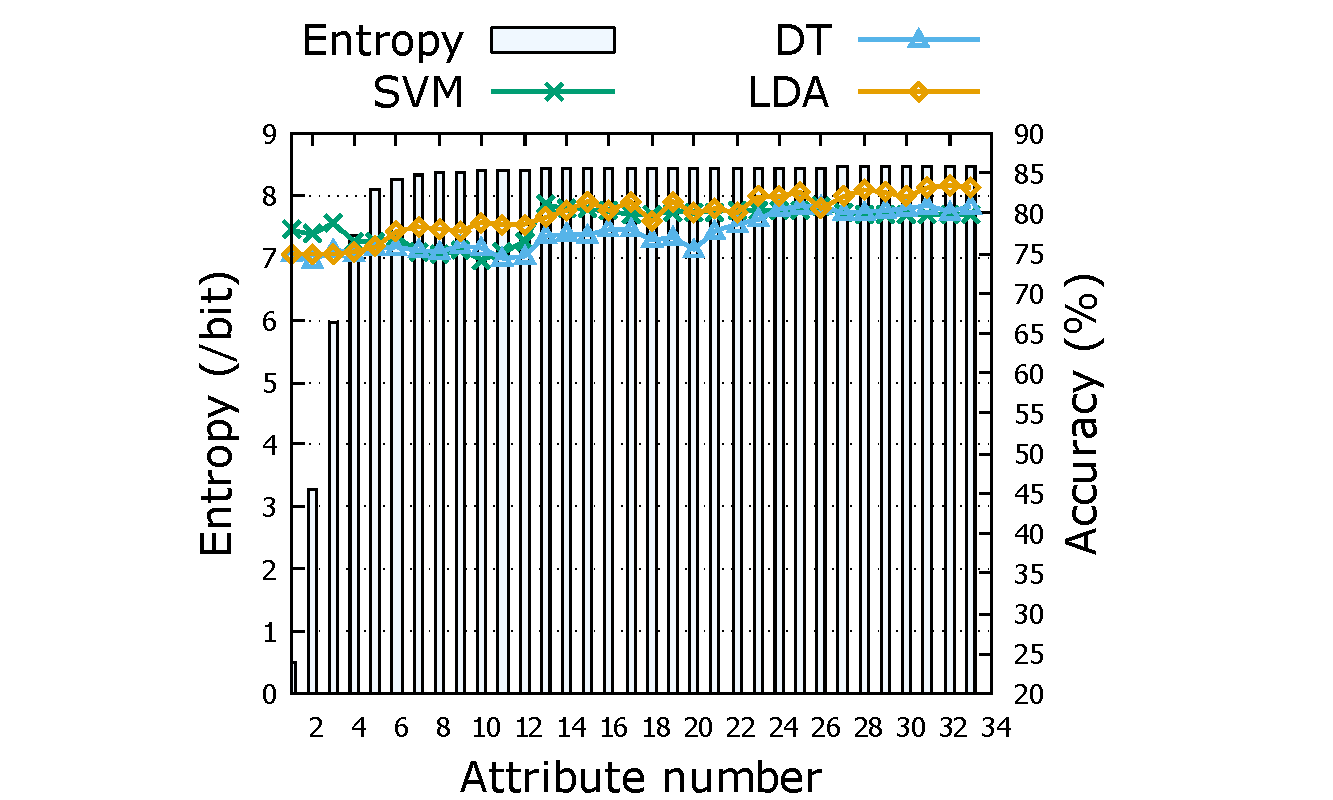
\includegraphics[width=0.6\textwidth]{chapter3/ionosphere_experiment_2_with_3_classifiers}
	}
\bicaption[fig:exp2_1]{基于属性划分的元组集合实验结果1}{基于属性划分的元组集合实验结果1}{Fig}{Testing results on attribute-based tuple sets}
\end{figure}

\begin{figure}[h]
\centering
	\subfigure[vehicle]{
		\label{fig:evehicle_exp2}
		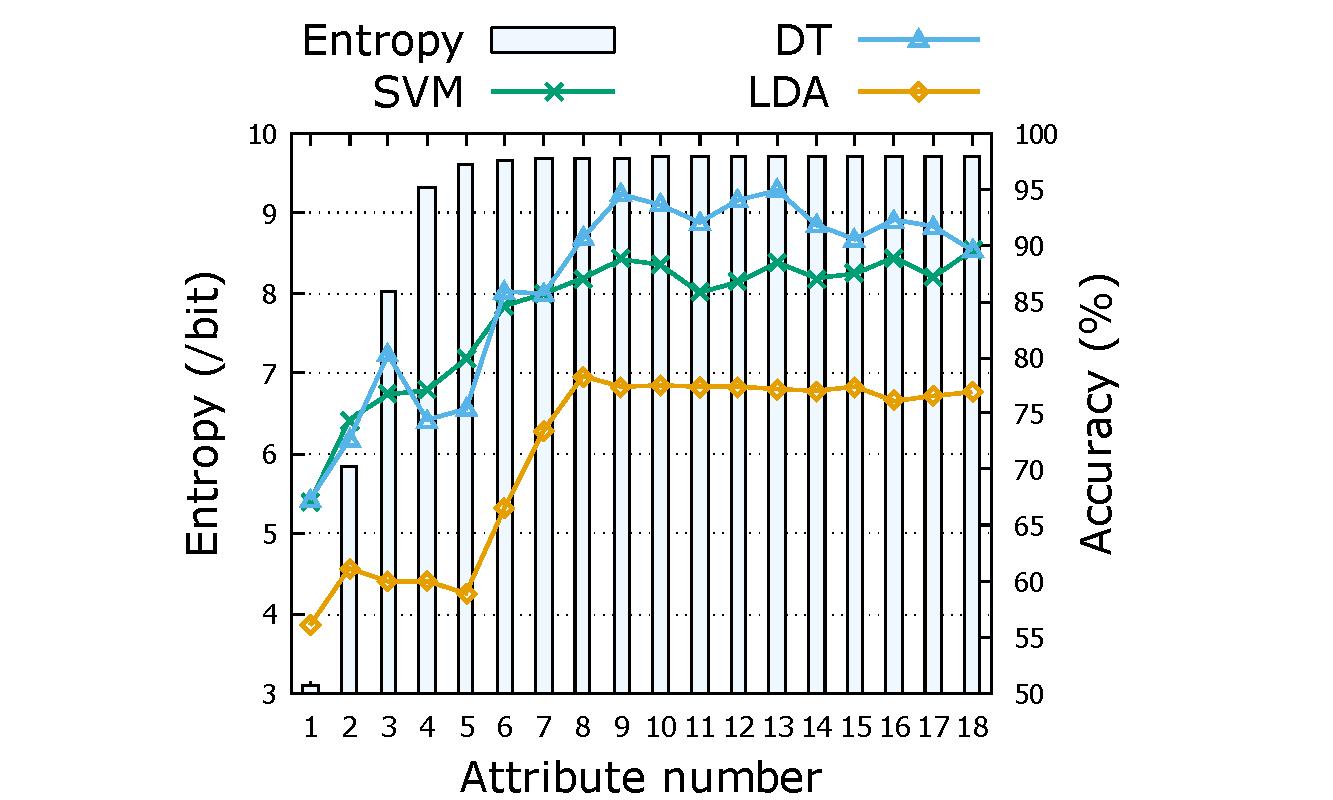
\includegraphics[width=0.6\textwidth]{chapter3/vehicle_experiment_2_with_3_classifiers}
	}
	\subfigure[letter]{
		\label{fig:letter_exp2}
		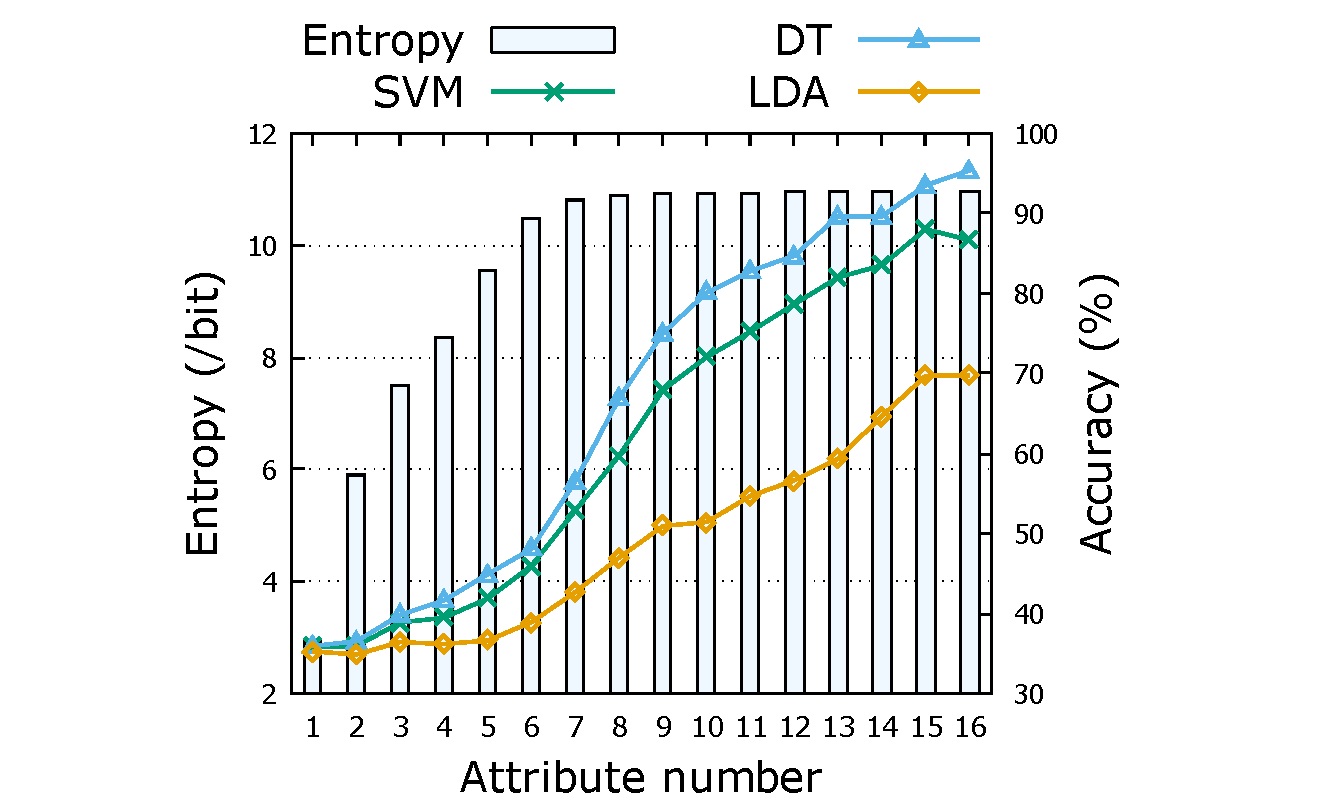
\includegraphics[width=0.6\textwidth]{chapter3/letter_experiment_2_with_3_classifiers}
	}
\bicaption[fig:exp2_2]{基于属性划分的元组集合实验结果2}{基于属性划分的元组集合实验结果2}{Fig}{Testing results on attribute-based tuple sets}
\end{figure}

\begin{figure}[h]
\centering
	\subfigure[mushroom]{
		\label{fig:mushroom_exp2}
		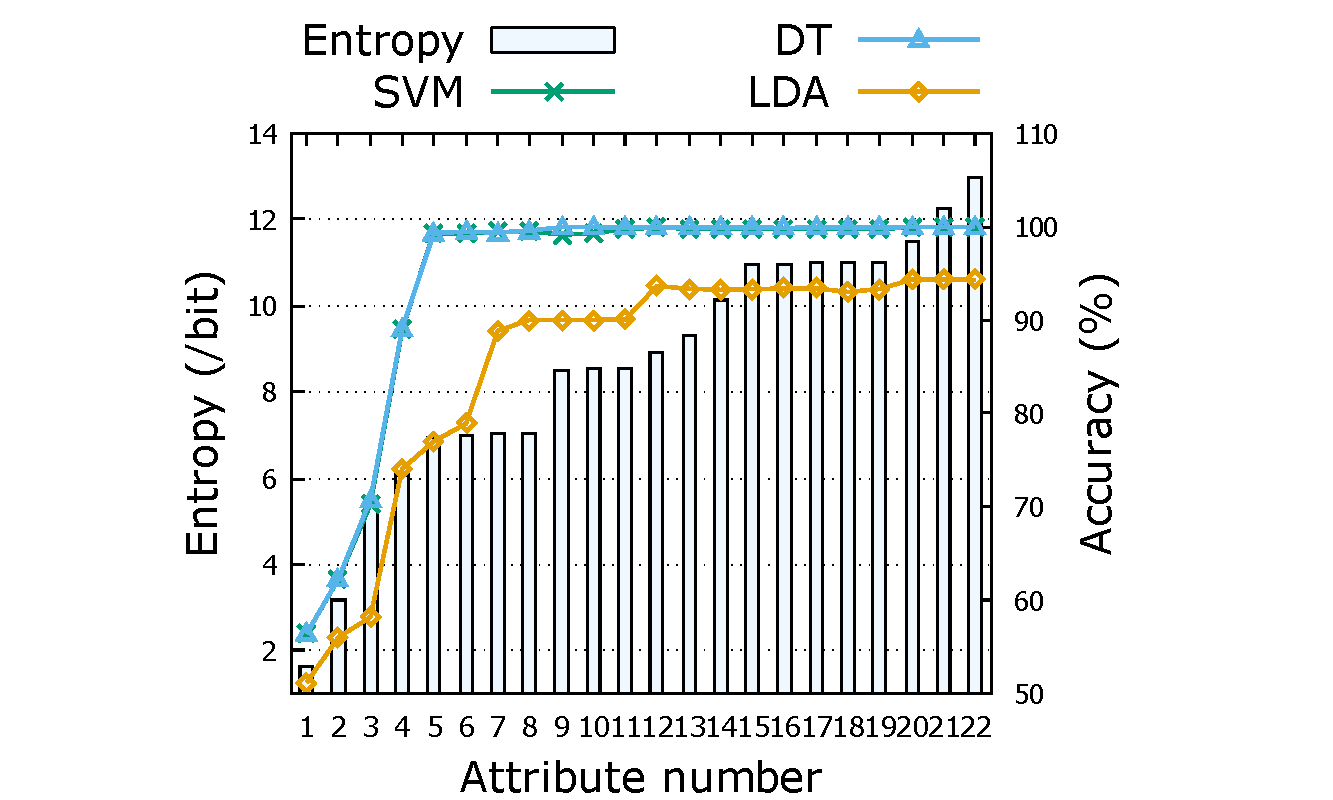
\includegraphics[width=0.6\textwidth]{chapter3/mushroom_experiment_2_with_3_classifiers}
	}
	\subfigure[nursery]{
		\label{fig:nursery_exp2}
		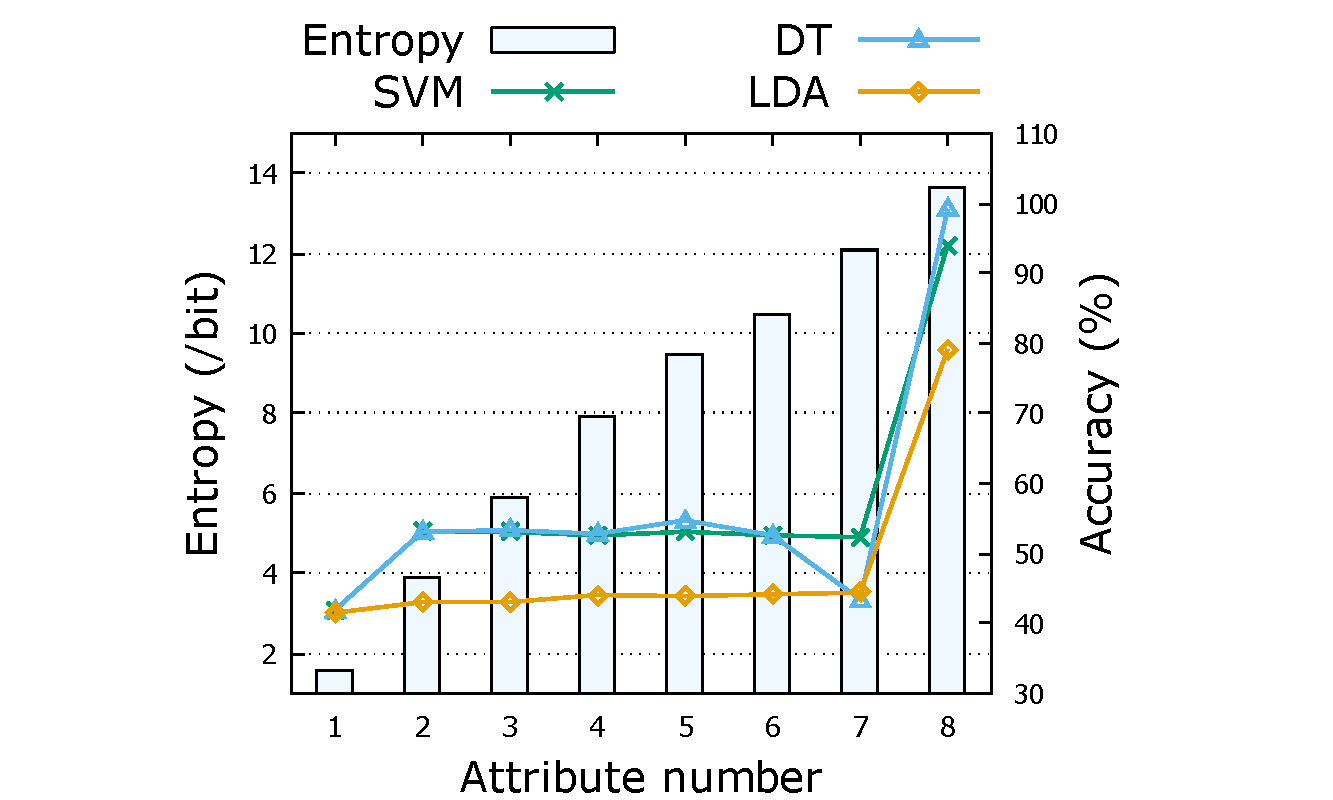
\includegraphics[width=0.6\textwidth]{chapter3/nursery_experiment_2_with_3_classifiers}
	}
\bicaption[fig:exp2_3]{基于属性划分的元组集合实验结果3}{基于属性划分的元组集合实验结果3}{Fig}{Testing results on attribute-based tuple sets}
\end{figure}

连续型数据集ECO,ION和VEH的实验结果被呈现在图\ref{fig:ecoli_exp2},\ref{fig:ionosphere_exp2}和\ref{fig:vehicle_exp2}中。根据这些实验结果,我们可以发现数据信息熵是随着属性数的增大而单调上升的。而图\ref{fig:ecoli_exp2}和\ref{fig:vehicle_exp2}可以看出分类器的分类正确率曲线呈现上升趋势,而图\ref{fig:ionosphere_exp2}呈现相同的趋势但是伴随着更多的扰动。尽管不同的分类器的表现有些许不同,但是这三个分类器的分类正确率都是随着数据信息熵的增加而上升。而离散数据集LET,MUS和NUR的实验,其结果被记录在图\ref{fig:letter_exp2},\ref{fig:mushroom_exp2}和\ref{fig:nursery_exp2}中。正如在图\ref{fig:letter_exp2},\ref{fig:mushroom_exp2}和\ref{fig:nursery_exp2}看到的那样,在离散数据集上的实验结果是与连续型数据集的结果很相似的,甚至更好一些。需要指出的是,在图\ref{fig:mushroom_exp2}中,其实是有三条分类正确率曲线的,但是决策树的分类正确率曲线被支持向量机的分类正确率曲线遮挡住了。相比于连续型数据集的结果,离散数据集上训练的分类器的分类正确率曲线也是随着数据信息熵的增大更上升但是更加稳定。

\subsubsection{基于记录划分的元组集合的实验}

\subsection{在大规模工业数据集上的实验}

\subsection{定价函数}

\section{本章小结}